\documentclass[border=10pt]{standalone}

\usepackage{tikz}
\usepackage{tikzsymbols}
\usetikzlibrary{calc,patterns,shapes.geometric}

\def\centerarc[#1](#2)(#3:#4:#5){\draw[#1] ($(#2)+({#5*cos(#3)},{#5*sin(#3)})$) arc (#3:#4:#5);}

\begin{document}
	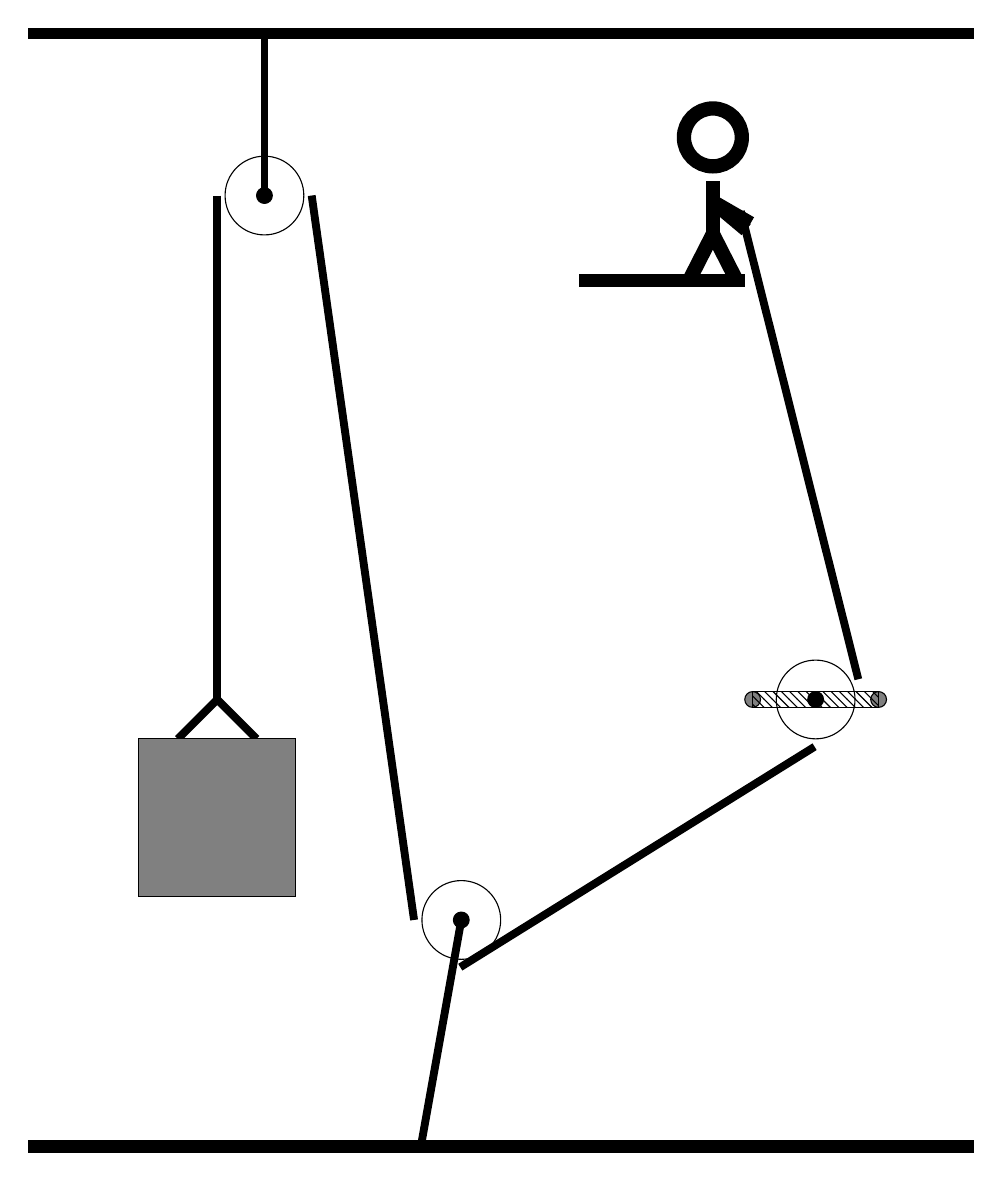
\begin{tikzpicture}
		%%%%% START %%%%%
		\draw[fill=black] (-2, 14) rectangle (10, 14.125);
		
		\draw (1, 12) circle (0.5);
		\draw[fill=black] (1, 12) circle (0.1);
		\draw[line width=1mm] (1, 14) -- (1, 12);
		
		\draw (3.5, 2.8) circle (0.5);
		\draw[fill=black] (3.5, 2.8) circle (0.1);
		\draw[line width=1mm] (3.5, 2.8) -- (3.0, 0);
		
		\draw[fill=white](8, 5.6) circle (0.5);
		\draw[fill=black] (8, 5.6) circle (0.1);
		\draw[fill=black!50] (8.8, 5.6) circle (0.1);
		\draw[fill=black!50] (7.2, 5.6) circle (0.1);
		\draw[pattern=north west lines, pattern color=black] (7.2, 5.7) rectangle (8.8, 5.5);
		
		\draw[line width=1mm](-0.1, 5.1) --  (0.4, 5.6) -- (0.9, 5.1);
		\draw[fill=black!50] (-0.6, 5.1) rectangle (1.4, 3.1);
		
		\draw[line width=1mm](0.4, 12) -- (0.4, 5.6);
		\centerarc[line width=1mm](1, 12)(180:0:0.6)
		\draw[line width=1mm](1.6, 12) -- (2.9, 2.8);
		\centerarc[line width=1mm](3.5, 2.8)(180:300:0.6);
		\draw[line width=1mm](3.487, 2.2) -- (7.987, 5.0);
		\centerarc[line width=1mm](8, 5.6)(300:390:0.6);
		\draw[line width=1mm](8.542, 5.857) -- (7.05, 11.8);
		
		\node at (6.75, 12) {\Strichmaxerl[10][-220][-30]};
		\draw[fill=black] (5, 11) rectangle (7.1, 10.85);
		
		\draw[fill=black] (-2, 0) rectangle (10, -0.15);
		%%%%% END %%%%%
	\end{tikzpicture}
\end{document}